\documentclass{report} 
  \usepackage{graphicx}
  \usepackage{lscape}

  \begin{document}
  
  \title{Multi-Robot Human Communication}
  \author{Maciej Musialek}
  \maketitle

  \tableofcontents

  \chapter{Introduction}
    Communication has been a subject of research for a long time now. With the development of computers and robotics a new area was opened regarding communication between humans and robots. With the addition of job automation allowing robots to perform tasks on their own and take instructions, the communication started playing an even bigger part in job distribution. Humans handle the job distribution and robots would perform tasks carried onto them.

    This project focuses on turn-taking communication for energy limited robots with an addition of trying to give some decision power to robots, like proposing potential moves rather than list all of them. It focuses on creating a robot platform with a user interface that will allow testing how single human interaction can improve multi robot collaboration. This will be done by comparing different levels of freedom to robots from no control to complete control over the environment and their choices. This was largely motivated by a paper done by Sklar and Azhar\cite{Elizabeth} in their paper on Argumentation-Based Dialogue Games for Shared Control in Human-Robot Systems.

    The aim of their project was a proposition of human-robot dialogue that would give an outline to how such communication could be implemented. With this a proposition of such communication was given with different layers of communication taken into account that describe the dialogue. In further research using their system, the researchers found that humans trust robots more with their decisions when such dialogue is implemented.

    This leads to the main motivation of the report, which is to develop a real time version of the dialogue system where robots interact with a human team to give even a better picture of how this dialogue can affect decisions made by humans. Such an environment could shed more light in argumentation research where in certain scenarios trusting the robot more in the environment could be of key to maximizing results. Such situations could involve search-and-rescue missions where quick correct decisions need to be made in order to maximize the number of victims saved and argumentation from robots could pose an ideal scenario for when humans give in to the pressure and machines can still do the calculations.

    One last motivating factor for the project is that robotics is a growing field of technology that is getting more accurate every year. Robots are beginning to recognize objects, with recognition that could soon approach human perception and later on go beyond it. In such a situation, having strong research done in human robot communication could pave the way for quick implementations of systems where situations might require a more focused approach. This can range anywhere from search and rescue to self-aware cleaning robots at homes that propose which rooms are the dirtiest by a quick glance of each of them.

    This leads to a conclusion that a framework needs to be developed for real time simulation of robot environments with dialogue plugins being inserted to suit the researchers needs. For this project, a stack of software will be created ranging from back end Robot Operating System simulation software to a Graphical User Interface that tells the user where each robot is and allow commands to be given for specific robots. Such an environment is going to focus on allowing maximum freedom to the researchers to ensure that their dialogue research is only limited by what kind of dialogue system they would like to set up.

    The main challenges with creating such a diverse system is in creating an environment where a variety of dialogues can be ran and tested. To achieve this, a modular system of classes needs to be developed to allow researchers to swap in and out different models of communication they would like to test on their users. It does not however suffice to simply create a dialogue class. To save time in future research, a unified environment has to be created to save time in reinventing a wheel for creating various scenarios to be tested. In this project, an environment based on Sklar and Azhar’s treasure hunt game will be implemented and ran along a modular communication class that will be fully editable by the user to ensure various models of communication are allowed. This will pose an additional challenge of creating a platform that holds the simulation software as well as the Graphical User Interface that are both in their essence modular inside the system. For this purpose, Robot Operating System(ROS) has been used to create a simulation platform and the main challenge with this is creating an environment that is also scalable based on the needs of research.

    The next sections of the report will focus on giving a concrete description of how this system was developed and how researchers can use it to help their work.

  \chapter{Background}
    Before setting off to outline what has been finished in the project and how certain choices were made in comparison to others, the report will be discussing the current situation of the robotics community and the human-robot collaboration in general for how the robots communicate with each other. Also a more detailed outline onto the treasure hunt game will be given to give a better image of why this research was chosen over others.

    With this in mind, it is important to outline what ideas are currently looked at and how they influence the field of robotics and more importantly, what they bring to the project. In the following sections, an outline of the treasure hunt game along with two main areas of research in robotics that are relevant to this report will be given. These evaluations will be concerning human-robot collaboration and research that was focused around the ROS environment.

    \section{Treasure Hunt Game}
      Following the introduction that said that this report will focus on creating a treasure hunt game, it is important to understand the concepts behind the game. The games aim is not to create a competitive game where users will interact. The main goal is to test the communication between various robots. With that said the following explanation will give an outline to how the game works and this explanation is directly inspired by Sklar and Azhar’s paper on ArgumentationBased Dialogue Games for Shared Control in Human-Robot Systems.

      The game works by using a simulation environment between a robot and a human. In this environment there is a map with hidden treasures, a robot that explores it as well as a human suggesting where the robot should go. The person that controls the robot gives commands as to which room the robot should visit first along with an option to ask the robot for its opinion on the matter. This gives room to possibilities of dialogue communication between two parties and as such give a robot the chance to persuade the user towards a better option.

      There are numerous possibilities for the treasures and their identification is important to yield different results as well as to use as little energy as possible to get a maximum score. This score can then be evaluated to see how the robot influenced the user and how the communication influenced the experience for the human as well as the score. This then can be used to decide the best strategy for dialogues. The possibilities for treasures can be demonstrated by a figure taken from Sklar and Azhar’s paper[1] which can be found below for ease of access.

        \begin{figure}[!ht]
          
          \centering
            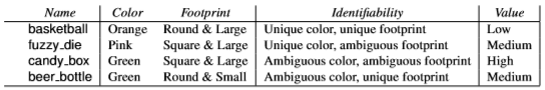
\includegraphics[width=1.02\textwidth]{figures/treasures.png}
            \caption{Example of Treasures in the game.}
        \end{figure}

      With these treasures it is easy to see how users might make errors between treasures that carry high ambiguity but also shows how it is unnecessary to use up energy for taking pictures of treasures that have very unique qualities and with that, can be simply grabbed for increasing the score. This could be developed in the environment to ensure that the robot makes sure that the user is certain of taking pictures of treasures that are implicitly unique.

      The game also makes the robot energy a precious resource with robot losing energy for practically every action that it takes apart from communicating with the user.

      This leads to the motivation in this report of creating this environment with customizability of Dialogues as well as ensuring that a multi robot environment is allowed to further see how increasing the number of robots affect the dialogue experience in Human-Robot communication.

    \section{Related work in Human-Robot collaboration}
      Currently research is greatly focused on human-robot collaboration for humans and robots in the same environment, working simultaneously on a task together. This in turn makes the current problem more unique. The problem we consider in this paper works on the assumption that humans and robots are in separate environments, and with that the robot can potentially have a lot of control over the environment. The following subsections give a more precise background in research of human-robot collaboration.

      \subsubsection{Same space collaboration}
        In their papers Liu et al.\cite{ChangLiu} and Govindarajan et al.\cite{Vijay} discuss collaboration in same space. 

        In the first paper\cite{ChangLiu} the collaboration is outlined by robot working together with the human. The setup of the experiment was to give each human-robot team a group of tasks that either required one agent to complete or a joint task for both of them. The aim was to finish a list of tasks as quickly as possible. The measurement parameters were mainly the fluency of collaboration outlined by Hoffman's metrics. Their results found many conclusions; one of which was that humans preferred working with robots that could infer plans based on human movement. This gives an implication to the project that ultimately guides the project to try and develop a robot that could propose movements as to giving the human full power over the environment and the process. In that way it can be considered good practice to let an idle robot move based on its own path planner to the closest room if it was neglected. This of course, is subject to human preference but allowing such functionality could be considered.

        In Govindarajan et al's\cite{Vijay} paper the main focus of research was search and rescue actions where robots infer different paths from where the human is headed thus maximizing the search space of a room. To develop an algorithm that would handle the robots, the researchers used the ROS platform. In their results they have found that using complementary homotopy classes for intelligent path finding increased the performance of robots helping them make more intelligent decisions. While not particularly useful for robots that search different rooms, using homotopy classes for finding out which robot should potentially reach specific rooms could be useful when making plans that revolve around finding maximum number of rooms helping robots achieve more efficient paths. Additionally another area of research would be with large amount of robots. In that research the robots would use homotopy classes to make decisions based on first movements of robots to try and predict which would be the next rooms that the current robot would choose. With that, the robots would move away from that area that will potentially be visited anyway to start exploring other areas.

      \subsubsection{Spatial recognition}
        Goto et al.'s\cite{Hiraki} paper work on maximizing fluency in human-robot collaboration and identifying challenges posed by robots when it comes to recognizing parts that would be required for assembly of parts. To achieve this they focused on a finite state machine approach for robots to help with table assembly. This can be considered a more limited approach in terms of robot intelligence since robots are limited in the amount of states they will be in. In their results they managed to see limitations with the robot both recognizing the human action and with the scalability of the software due to most of it being hand made beforehand. The paper mainly focused on being able to achieve the task in comparison to achieving the task efficiently or effectively. With that in mind it poses considerations that need to be taken when looking at robot design one of the most important being a challenge being the robot understanding what it sees and how limited they can be when it comes to object recognition.

      \subsubsection{Modalities of human preference}
        While in their paper Fiore et al.\cite{Fiore} did not use the robot operating system, they embarked on a task that would prove that robots are capable of completing collaborative tasks based on human supervision. In this sense, their paper is very related to research outlined in this paper. Fiore et al. Propose a complex system that is built on sophisticated software for intention inference, path planning, task execution and communication. In their results they have proved that the system is capable of: handling joint goals and actions, handling users preferences, handling agent beliefs and monitoring human actions. With that in mind, a multitude of research has been proposed in creating human-robot collaboration and proving that the tasks are in fact possible complete.

      \subsubsection{Conclusion}
        It seems that a lot of current research has put a great focus on proving that human robot collaboration is indeed possible with a huge variation of approaches between each paper. While quite a new area, it is important to note that currently, there doesn't seem to be a greater standard in how research is carried out with researchers assembling software based on their research preference. It does not dispute the fact that every research paper proposes new considerations in human-robot collaboration and that possible improvements are drawn based on their approaches.

        This leads to a conclusion that Human-Robot collaboration is a very undeveloped field and will start presenting more exciting opportunities in the future for researchers to look at. Currently it seems that a great deal of effort is in ensuring that fluency between agents is maximized making the experience faster and more enjoyable for the participant in the study and potential agents for developed systems in the future.
    
    \section{Research in ROS environment}
        The reason for choosing to research ROS in greater detail is that it will be the main platform that runs the robotics simulations in this Project. In essence, it will be the backbone of the system and a lot of work will be determined by the success of its implementation. To achieve this, a solid background on how it was used in the past and what it has been used for is considered to ensure that the wheel has not been reinvented as well as to see potential uses of ROS to later on expand the system when it is developed.

        In comparison to previous research that focused on proving various possibilities of robotics systems, research that focuses on using ROS environment is mostly aimed towards developing various frameworks to ease the use of the environment to achieve certain results. As such, it can be compared to human-robot collaboration research as focusing more on solving problems than proving. Following sections outline various works that used the ROS environment to achieve their goals.

      \subsubsection{Frameworks}
        In their two papers Fok et al.\cite{ChienLiang} and Liang S Ng et al.\cite{Liang} focus on creating two separate networks that provide an interface for grabbing robots and control for complex whole body robots with multiple parts. In both of the papers, ROS was being used which stands to justify just how powerful ROS can be in manipulating various environments. In fact, the paper on creating a hardware and software problem for intelligent applications, is very similar to the approach this report is focused on. The simulation platform is in fact exact with the only difference being controlling single robots forwards and backwards rather than using path planning for the problem. From these findings, given time, the report can be further studied to include complex body robots that can be controlled over the cloud with hand held devices. This only signifies the availability of technology for implementing complex robot systems using ROS.

      \subsubsection{Domain specific research}
        Deusdado et al.'s\cite{Pedro} research focused on creating an aerial-ground teams in ROS for systematic soil and biota in estaurine sampling. Mario Vieira et al.'s research further focused on creating applications for monitoring human daily activity and risk situations in robot-assisted living. Both of these papers can be considered extremely centered around the areas that they focus on and show the variety of scenarios that ROS can be used for. Both teams achieved great success in their plan to centralize use of ROS for their respective goals and showed how useful they can be in further research. The first paper gives us an idea of how ROS can be used to implement robot teams, giving us ideas about how to space out cloud platforms to further enrich the environment while the second, allows us to see how to use robot sensors to view activity of humans. 

        This knowledge, can in fact be extrapolated to the project in future works to give a richer environment. One where each robot is directly responsive to actions of the other through the use of sensors rather than shared goal reaching creating a more human like collaboration not only between the robot and the human but throughout the whole team. It is important to note that while right now the robots focus is to reach desired destinations and share data to produce better maps. An alternative of proposed research above shows us that using a more intuitive approach can be just as useful.

      \subsubsection{Conclusion on ROS research}
        It is very easy to see that ROS research and implementations revolves around creating better frameworks and centralized domain problem solving. It is a very young field that so far didn't set standards towards what would be the best approach so that researchers could start tackling these issues and start improving on standard solutions. This in turn, emphasizes that the field is going to expand creating more elaborate solutions and frameworks for specific domain problems. At the time this report was written, most papers presented here are papers that came out in 2016th to ensure that the image of current affairs is as accurate as possible. With this information, as presented above ideas can be drawn about possible improvements to the implementation that could in turn create an environment where the collaboration is as fluent as possible with robots taking same type of initiative that normal humans would.

      \section{ROS challenges posed by its creators and community}
        Currently ROS is an overwhelmingly expanding software with new additions being added. ROS started in 2010 and already had 9 releases with the 10th coming out in May 2016. This sort of expansion rate pushes developers to re-learn the structure and standards set by ROS every few months, in turn making the frameworks obsolete every 8 months or so IF they used code that ROS creators deemed unnecessary in future releases or made it deprecated through certain decisions. This challenge is actually an obstacle for ROS creators themselves as in some examples, the Wiki pages can reference functions that can be considered deprecated in future releases. This in turn makes developers turn to the ROS community which is limited to the small group of robotics specialists using ROS that are willing to help on answers.ros.org.

        The community itself is compromised of a fairly small amount of user group that cannot be compared to regular software developer websites like StackOverflow or BigResource where commercial development and advice seeking can start to compare itself to a competition of its own. This produces problems when a regular developer that didn't have much experience with the environment, thus making it harder to develop in this network.

        It is also extremely important to note that at this point in time there is a huge deficit in the amount of available resources the developer can reference to when it comes their struggles. The few books that do exist to help users develop their knowledge are few and their knowledge as previously stated can become obsolete extremely fast due to ROS's quick expansion rate. When this report was created, there were also no current frameworks available for faster safer development or third party libraries to help a developer create a bigger understanding which means that the wheel of development for ROS is mostly reinvented every time a new idea is presented for development. This leads to a conclusion that the outlined specification will be extremely challenging posing a lot of stalls for implementation of the software.
        
    \section{Conclusion}
      It is clear that ROS is an amazing platform offering its users a great diversity in use. The research in human-robot collaboration and ROS is starting to expand the use of ROS in human-robot collaboration is starting to slowly become a standard. This in turn means, that selecting ROS as a developer platform for robot simulation is definitely a right fit for this project.

      With the previous section, it is clear that there will be challenges in this project that might in fact not get fulfilled simply due to lack of resources that will be able to acquire and through that, a careful consideration will be taken to ensure that the goals are realistic and not reaching outside the scope of the possibilities.

  \chapter{Specification for the report}
    To ensure a good outline of the project is given specification needs to be provided for various parts of the system to later on lead the design, implementation and testing of the environment. The following sections break down the system into its biggest parts and give a set of requirements as guidelines.

    \section{The simulation environment}
      The robot environment will be the center of emulating the environment. It will be responsible for housing the Robot Operating System server with maps, odometry for robots and mapping the robots inside a map so that they will be able to move around and accept commands from outside sources i.e. the GUI and transfer these commands into robot movement and task allocation. Below is the outlined specification for the environment.

      \begin{itemize}
        \item \textbf{SE1}: ROS based simulation environment.
        \item \textbf{SE2}: An environment that allows simulation of a robot on a 2-D plane with the map received from project supervisor.
        \item \textbf{SE3}: Accepting commands from outside sources that guide the robot e.g. Go to room 1.
        \item \textbf{SE4}: Responding to commands about robots position and whether it reached its goal.
        \item \textbf{SE5}: An ability for the robot to realize which rooms are closest to it.
        \item \textbf{SE6}: Robot is able to find its own way inside the map to the goal.
        \item \textbf{SE7}: Allow for more than one robot in a single simulation.
        \item \textbf{SE8}: Robot is fully aware of another robots presence.
        \item \textbf{SE9}: Robot is able to avoid collisions with other robots.
        \item \textbf{SE10}: The environment can accept various maps and robots can adapt to these.
        \item \textbf{SE11}:  (Optional) Simulation minimizes the use of system resources.
      \end{itemize}

    \section{Graphical User Interface}
      The Graphical User Interface is a crucial aspect to how the task distribution will be managed. Whether it is click and go or hot keyed commands is a question that will be crucial here. The human factor needs to be taken into account as basis for testing but having a user interface that doesn't allow comfortable work will only result in slowing down the human factor and making the results biased towards the robots working by themselves. Below is the outlined specification for the GUI.
      
        \begin{itemize}
          \item \textbf{UI1}: Interface should provide an approximated view of the simulation.
          \item \textbf{UI2}: Interface provides options for users to select rooms that robots go to.
          \item \textbf{UI3}: Users are able to select robots that they want to send goals for.
          \item \textbf{UI4}: User has the option of grabbing the treasure, taking the picture and moving on.
          \item \textbf{UI5}: Upon receiving the picture user has the option to take the treasure.
          \item \textbf{UI6}: Interface contains the map with an outline of rooms.
          \item \textbf{UI7}: Interface updates robots positions on the map based on where they are in the simulation.
          \item \textbf{UI8}: Interface accepts various Dialogues when a command is executed to show to the user.
          \item \textbf{UI9}: (Optional) Keyboard shortcuts implemented to smooth out the job as opposed to point and click where a mouse has to move all the time.
        \end{itemize}
    \section{Dialogue Interface}
      Testing the environment that was developed to the specification is the main focus of this project. It is however important to ensure that various models of communication are allowed to be ran to make the system usable and fulfill its purpose as research assistance and possibly assistance in the future for developing systems. Below are some main requirements for the dialogue interface.

        \begin{itemize}
          \item \textbf{DI1}: Hold necessary dialogues for different scenarios(Select room, Take a picture, Take treasure)
          \item \textbf{DI2}: Cater to different amounts of responses.
          \item \textbf{DI3}: Be outside of the GUI to ensure modularity.
          \item \textbf{DI4}: (Optional) Allow an array of responses for a given action(Two different sentences for the same action).
          \item \textbf{DI5}: Dialogue possibilities held on an external file.
        \end{itemize}

  \chapter{Design}

    The systems goal is to simulate a robot environment with multiple possible robots on the platform. It also has to provide researchers with the chance to edit the dialogue environment freely with different modes of communication. To achieve this, the system needs to have back end simulation software which in this case is going to be implemented in ROS environment. Following that, the ROS operating system will need to be able to connect to a server so that it can accept external commands and finally, it needs to boast an easy to use GUI that connects to the server and needs to be able to send and receive commands to and from the server. The server code is implemented by the supervisor of this project Sklar and does not need to be a part of the design but will need to be included as consideration when designing the system.

    The following sections outline the main modules of the system and consider different alternatives for the design.
    \section{Protocol for communication}
      It is important to outline the protocol for the communication. The system boasts a complex approach where different components connect to each other and with that, setting the communication protocol from the start will ease the design considerations in the future.

      The center of this implementation is the server that handles the traffic in the environment. It allows communication between various nodes and specifies the name convention for various parts of the system. This naming convention allows anyone troubleshooting the server to be able to see where the fault is. This naming convention suggests various for the system which are(For further explanation refer to the technical review provided in \cite{technical}):
        \begin{itemize}
          \item \textbf{SimR}: The simulation environment on which the robots operate.
          \item \textbf{TabUI}: The interface on the user side that controls the simulation environment.
          \item \textbf{Hider}: Class responsible for hiding and presenting treasure information.
          \item \textbf{Server}: The center of the application that passes messages through and ensures connections are valid. 
        \end{itemize}

      The main communication will revolve around the Server node and as such following design for communication is proposed which is very closely related to the one outlined in the technical preview\cite{technical}:

        \begin{figure}[!ht]  
          \centering
            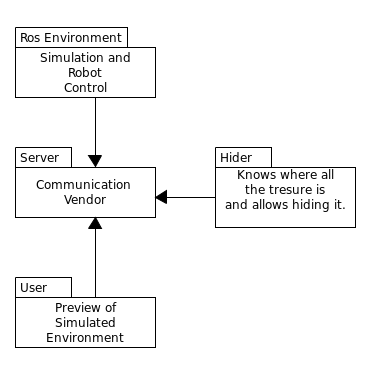
\includegraphics[width=0.7\textwidth]{figures/mainCommunication.png}
            \caption{Outline of the top level of communication.}
        \end{figure}

      With this main outline of communication done, it is also important to show how communication will be handled before it reaches a server. To do this the next two sections will talk about how communication is done in and out of ROS as well as how communication works in and out of the GUI.

      \subsubsection{Robot Operating system communication}
        ROS uses a published/subscriber mode of communication for its transfer of information. This means that while it is extremely simple to communicate between inside nodes, a new node will have to be developed that keeps communications to ROS to be switched on from outside sources. This can be viewed in the following figure:

          \begin{figure}[!ht]  
            \centering
              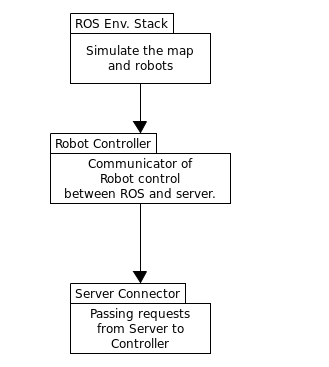
\includegraphics[width=0.8\textwidth]{figures/RosCommunication.png}
              \caption{Outline of the top level of communication.}
          \end{figure}

        The graph above presents a figure that shows that the communication starts at ROS Environment Stack. This has to be switched on for further channels that make sense. Then a robot controller node has to be created to ensure that sending goals is feasible when a command comes in but it shouldn't have direct connection to the server. The report has taken advantage of publisher/subscriber mode of communication and makes the server controller and robot controller contact in that exact manner. This actually allows for modularity between nodes as neither has to be switched on first and they can be changed and modified freely per users need. Considering that ROS codebase is done either in C++ or Python, with C++ proposing a better API in ROS environment, both nodes will be created using C++ and ran inside the same package that the simulation environment runs in to ensure maximum compatibility. This gives a good of idea of how the communication will be handled inside ROS. The next section will discuss how this communication is handled inside the Graphical User Interface environment.

      \subsubsection{Graphical User Interface/Hider Communication}
        In the Graphical User Interface, we can't take advantage of the Publisher/Subscriber approach that ROS loves to use. This means that while we can easily create both the user interface and the client that connects to the server. We need to think about how communication between the two will work to ensure that both writing and listening to the server is allowed and fires events based on responses. The same can be said for the Hider interface. This Hider interface could be implemented on the ROS environment stack alongside everything else but for the sake of modularity, the report will keep it outside. To develop this environment the following proposition is made for the environment:


        \begin{figure}[!ht]  
            \centering
              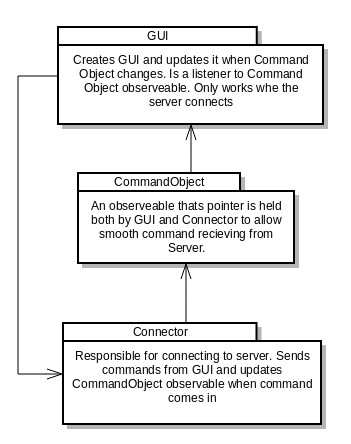
\includegraphics[width=0.8\textwidth]{figures/GUICommunication.png}
              \caption{Outline of communication inside GUI.}
          \end{figure}

        The Graphical user interface will implement an Observer design pattern to synchronize the communication between the GUI and the connector when a message comes in. The connector receives a command, changes the CommandObject and because the CommandObject was changes, the GUI as a listener will be fired and update the map. On the other side when the GUI wants to send a command, since it implements the Connector as a connection class, it should simply be able to pass the parameters directly into a command inside the Connector leaving the CommandObject strictly to the GUI to be fired when changed. With this, the report now has the design for the main protocol of communication and the next sections discuss the choices for design inside the ROS environment and GUI for the user.

    \section{ROS Environment}
      The most important consideration in design is scalability with which the simulations can run. In ROS we have two options for running the simulations one of which is Gazebo and the other Rviz for simulation preview. This is important to understand how the environment works and also if it actually works properly in terms of multi-robot environment.

      Each environment provides a certain ease of use inside the project with Gazebo allowing to build packages for robots making it a nice candidate for quick setup but also requires to constantly run Gazebo in the background which doesn't make it an ideal candidate for saving resources and performance which in the future might affect scalability. To avoid this issue, a better option would be to run Navigation Stack which is what will simulate the topics and the robot environment and to run Rviz for debugging purposes.

        \begin{figure}[!ht]  
          \centering
            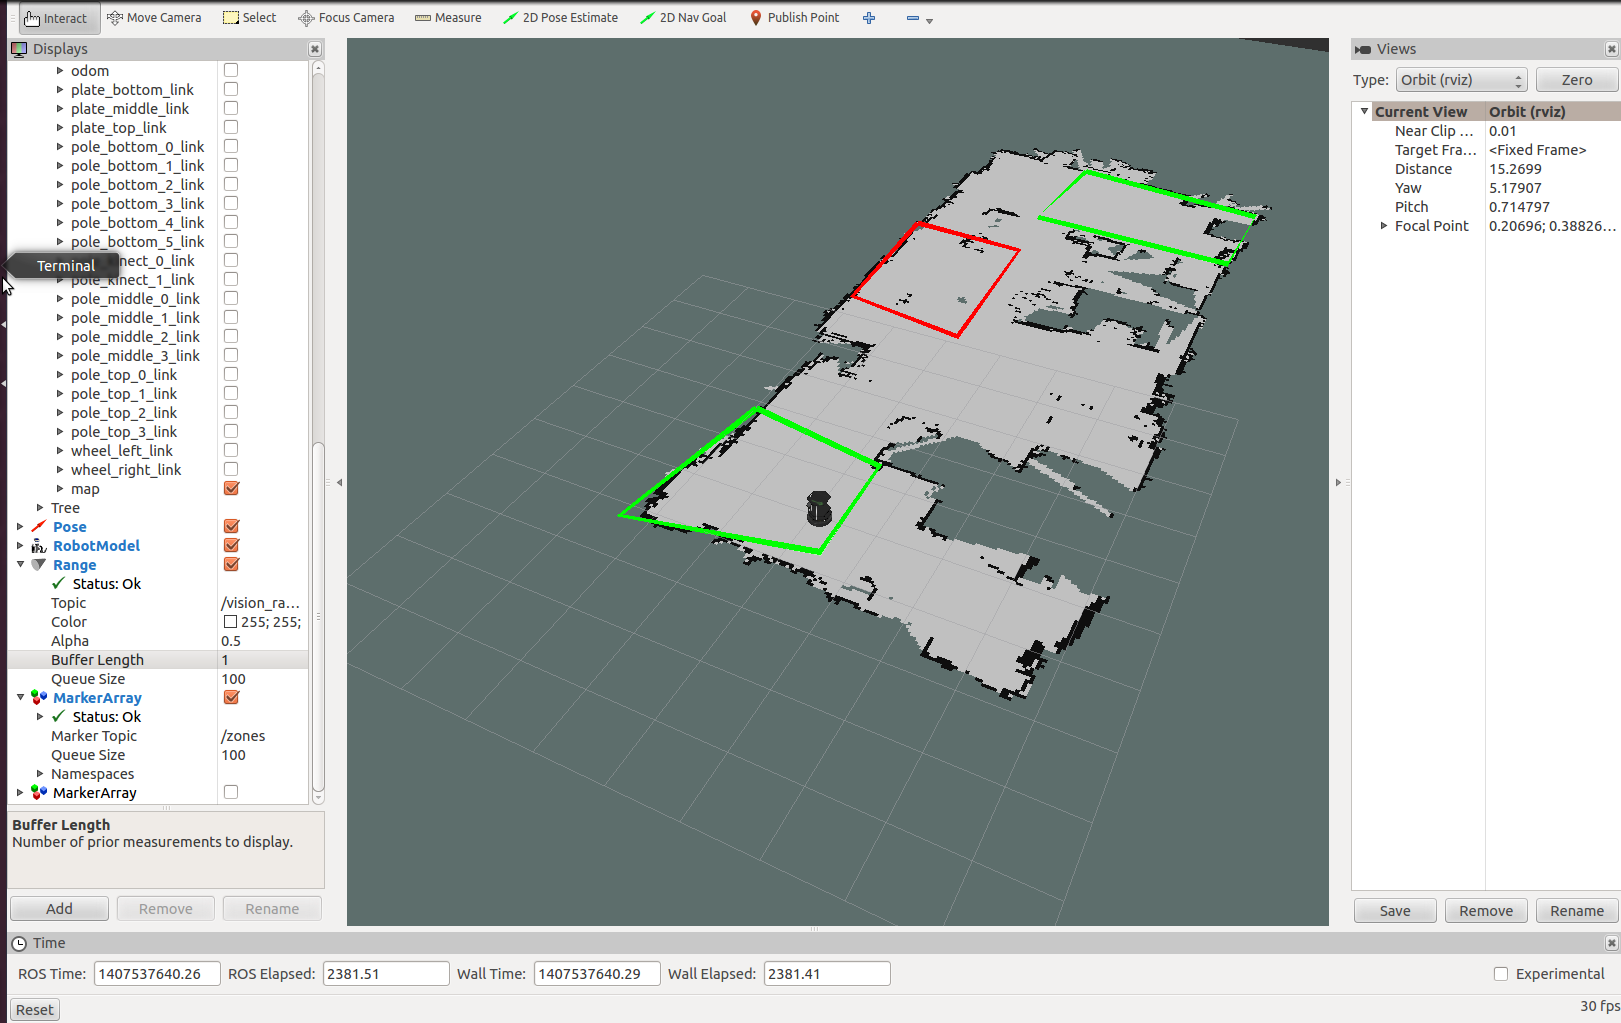
\includegraphics[width=0.6\textwidth]{figures/RVIZ.png}
            \caption{Example of Rviz running.}
        \end{figure}

      From current research, Rviz does not provide functionality in terms of displaying multiple robots but running it is optional in terms of environment so in that choice, Rviz is chosen to be the main simulation display in the first stages of the project. It will be used that when goals are set by the controller, the robot walks towards a certain path as well as ensure that the multiple layer design that ROS needs to implement in the navigation stack is chosen.

      To actually create multiple robot environment is a question of implementation and trial and error in the environment rather than design as the ROS navigation stack at this point is generally very unfamiliar however using answers provided in \cite{wiki1} we can imply that the design of the robot architecture will be as follows:

        \begin{figure}[!ht]  
          \centering
            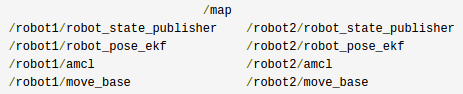
\includegraphics[width=1\textwidth]{figures/ROSPlan.png}
            \caption{Ideally how multi robot is going to work.}
        \end{figure}

      Figure above shows how two robots are mapped to the same map. The main challenge with this will be figuring out how to implement this in the Navigation stack without using gazebo for the backbone to avoid the need to consume extra resources through gazebo.

      It is important to note that originally the implementation will try to set up an environment with one robot that runs and allows to set up the GUI first. If however this doesn't pose too many issues, a two robot environment will be developed before the GUI is taken into consideration.

    \section{GUI for User and Hider}
      The GUI is the front of what the user sees and experiences through the use of application. This will be the main product that researchers will show to the users to later enquire about the dialogue model. It is therefore essential to ensure that the design is as simplistic and as intuitive as possible. After all the user should not feel like the design of the interface is in any way overwhelming. This could lead to not paying attention to the dialogue systems as well as bring on an experience that would otherwise compromise the flow of actions that lead the user from beginning to the end.

      While the previous section included an explanation of how the environment communicates with the server it did very little in explaining how the GUI is going to look or what programming language is going to be implemented to ensure both a pleasant experience for the user but also maximize compatibility with the Java Server that runs in the background and allows communication to the ROS environment. Both of these are discussed in the following sections.

      \subsubsection{The looks of the design}
        The application boasts quite a lot of information that the user needs to take in. The short list below summarizes most of the information that the user will see:
        \begin{itemize}
          \item The map and robots location on the map.
          \item List of possible robots that the user can select from
          \item Objectives of the game
          \item List of rooms that the robot can go to.
          \item Information about energy levels of various robots; each different.
          \item Dialogue windows popping up to start communication between robot and human.
        \end{itemize}

        With this list, a design can definitely start forming into shape with the last point being one of the most important ones. That the dialogues pop up rather than be placed in a sidebar or a top bar or anywhere else. The user should have a strong level of interaction with the robot as well as be able to make note of the communication that occurs. Once a robot gets a command it should communicate with the Human and notify them of possibilities or try to persuade them to do other things like go to another room or pickup a treasure that is distinct enough to others that it will be better to grab it rather than take a picture of the item if the user decides to take a picture of a distinct object.

          \begin{figure}[!ht]  
            \centering
              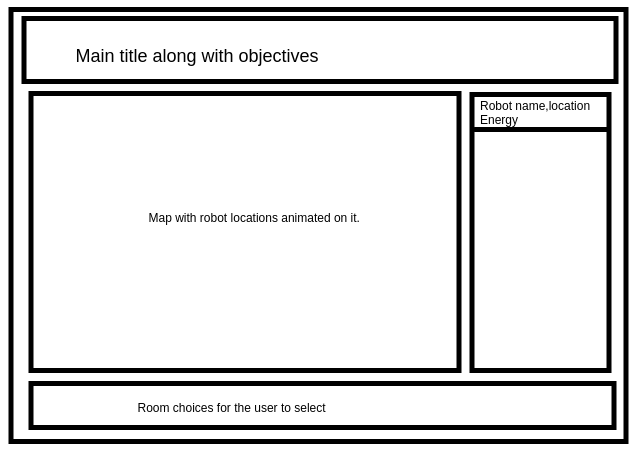
\includegraphics[width=1\textwidth]{figures/GUIDesign.png}
              \caption{Basic idea of the GUI design for the user.}
          \end{figure}

        This design largely represents the work flow of the application with the Dialogue window popping up requesting user input right in the middle of the frame to ensure that the user gives input to the robot and maximize the efficiency of the application.

        With regards to the hider GUI, it could be implemented as a GUI but creating a simple code that holds variables would make more sense as it will actually be faster to edit those than to do so through the use of GUI. It will keep external files to the minimum not requiring to run separate external files along with that .jar compiled file and with that rationale. At this point in the project it will suffice to have the Hider work at source code and change the variables inside it, compile and run accordingly.

      \subsubsection{Programming language choice}
        To develop the GUI itself, there are numerous options to choose from. Different languages offer different options and a list of possible programming languages taken under consideration in this report is:
        
          \begin{itemize}
            \item C++
            \item JavaScript
            \item Python
            \item Java
          \end{itemize}

        Each of these languages would be a good choice but to outline the main differences, each following chapter will discuss their positives and negatives.

        C++ is a great programming language for memory management and as such maximizing efficiency of the software through the use of pointers and memory dumping whenever any information is not necessary. With that, a graphical user interface could be set up in such a way that the user could execute a program and run it very easily. It does however bring a need to compile to specific operating systems like Linux, Windows or Mac depending on the platform that the software runs on\cite{cplus}. Also C++ has commands that are specific to each operating system meaning that while creating a C++ could potentially bring out the best performance, it would also create platform dependent binaries or even so, make code that is platform dependent and with that, it could potentially minimize the target audience for the project. Keeping the project as open platform as possible so that any user could run the GUI is also a very important aspect of the project.

        With JavaScript, the GUI would experience a very good boost in terms of GUI looks. Combining JavaScript with HTML could produce a very neat looking design that could update itself based on server output however the big issue with JavaScript is that it doesn't really support connecting to the server unless external platforms like socket.io\cite{socketio} are brought in. Otherwise JavaScript is AJAX dependent which means that it would either require an additional library importing and learning a new platform or, expanding the server to allow API calls but these kinds of implementations fall outside of the scope of possibility for this project.

        Python offers great ease of use, is a relatively fast language in comparison to the previously mentioned languages. It also works great with sprites and drawing GUI’s which could prove extremely useful in this project. This can be witnessed in books that teach Python programming and use sprite and GUI design as their main chapters\cite{python}. With python however, there is still an issue that was present with C++. While Python is an interpreted language, it works only if the interpreter is installed on the computer. With Linux based systems that is not an issue at all because Linux runs a lot of its software using Python so the interpreter is always pre-installed but when it comes to Windows, this interpreter is not installed as Windows tends to keep to its .exe file system and that again, would limit the scope for the audience.

        Java is the language that the Server was developed in. It is a language that has pre-built GUI libraries called Swing and AWT which allows for a fast GUI prototype implementation and is even use for general development in bigger corporations. These two are definitely favorable when it comes to the GUI created in this project. Java is also present on most PC’s because while systems don't use it as a pre-requisite, a lot of software is implemented using Java and there is a very high chance that any computer visited will have Java working on it. This provides a rationale for choosing Java for the implementation of the GUI.

    \section{Testing design}
      This project will taken upon itself a test driven development sprint where a set of criteria outlined in the specification will guide the way towards a successful implementation of the product. It is however important to outline some criteria other than the simplistic ones that are given in the specification for clarity purposes.

      One of these is to outline a use case for when the users are using the GUI to give an outline of what a successful implementation should do. With this user case, testing will later be carried out to ensure that the application has successfully undergone implementation purposes. Figure 4.7 demonstrates the basic use case that outlines the what the user should be able to do inside the application.

        \begin{figure}[!ht]  
          \centering
            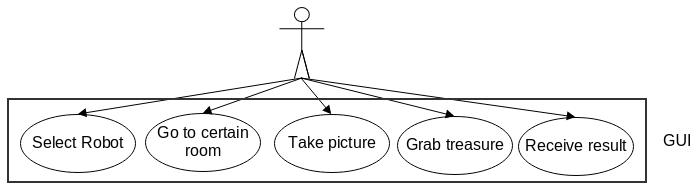
\includegraphics[width=1\textwidth]{figures/GuiUseCase2.png}
            \caption{Use Case for GUI.}
        \end{figure}

      With this we can see all the commands that are available to the user all of which should run successfully and without any issues.For a better explanation of the stages through which the application should go, a flow chart needs to be constructed. Such a flowchart will provide a better explanation of how the system works and in which areas lies logic that needs to be tested. Diagram presented in Figure 4.8 demonstrates the extent to which each logic function will need to be tested.

        \begin{figure}[!ht]  
          \centering
            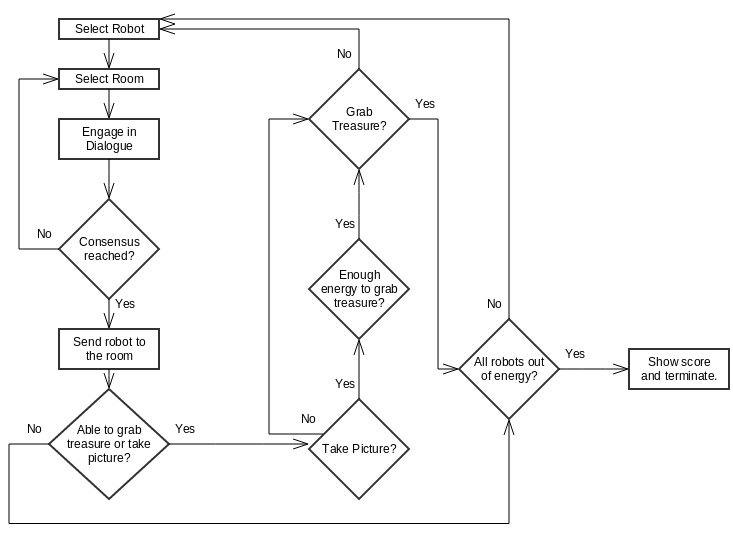
\includegraphics[width=1.1\textwidth]{figures/flowChart.png}
            \caption{Flow chart for GUI use.}
        \end{figure}

      It can be then implied that for the test driven implemented in this project, the application will need to teach the terminate state while ensuring that each decision in the use case has been tested. This will provide enough information to say that the product was fully finished along with the information provided in the specification.


  \chapter{Implementation}
    The fully implemented product has been derived by the guidelines received from Elizabeth Sklar, King's College London who guided the implementation of the report and provided a Server package that in turn is now the main communicator of information of the finished product. This product can be broken down into several components these being(For a better explanation please refer to figure 1):
    \begin{itemize}
      \item Simulation Environment - A composition of packages composed of: Server Control, Robot Control and Robot Simulation.
      \item Server - A package composed of communication protocol classes.
      \item Hider - Composed of classes responsible for server connection and Hiding the treasures.
      \item User - Composed of classes responsible for UI, server connection and Remote Robot Control.
    \end{itemize}

    In following sections of this report, a more broken down structure to provide insight into how each of these is achieved.

    \section{Simulation Environment}
      As stated before, the ROS stack is a combination of three packages. The Server control, Robot control and robot simulation. They interact with each other in exactly the way that was stated in the design with Server control connecting to the robot control that then sends commands to the robot simulation however a more precise definition will be given in the next sections.

      The implementation also makes use of launch files to reduce the number of terminals that have to run during the execution of the simulation environment. This is due to the fact that with just the launch files given in the ROS tutorials, the amount of windows that have to be open for executing the environment can increase quite exponentially with the number of robots and is in no way automatic.

      This launch file further lists the important packages that implement the simulation and exposes user to the outline of how the ROS environment operates with further explanation of packages outlined in next sections of the implementation chapter.

      \subsection{The Server Control}
        The Server control implementation is based around creating a serverToController package outside of the ROS simulation. This is done to ensure that a modular approach was taken and the server can be extracted and replaced if such a need occurs. It also takes advantage of publisher/subscriber method to implement a workaround Observer Design Pattern that allows two classes to work together using callback functions rather than the Observer fire() events and implementing extra interfaces. This in turn, creates a much simpler to work with environment where the communication between two classes is transparent and callback methods are limited in their simplicity. It also implements C++ threads to allow socket connectivity through clients thus allowing a C++ server to connect using TCP client to the Java Sever running on currently a local host machine.

        The server control also ensures that no commands that are irrelevant to the Robot controller are sent through. This includes commands like \%\%ack or \%\%ping that only need to be answered by the server control. This in turn creates a sieve for commands from the server with only useful ones going through.

      \subsection{The Robot Controller}
        The robot controller is inside the same package that the Server control is based in. This is mostly to ensure that while modularity is kept, the classes aren't spread out so far inside an environment that it would make it difficult to troubleshoot. Also since these two nodes have a ROS topic that is dedicated only to themselves, it makes sense that they would be stored inside the same environment.

        The controller is used inside the ROS environment to communicate between the server commands and the robots themselves that are simulated and switched on along the server control and the controller. This controller send information to robot\/move\_base\/goal to send the robot a goal command that they need to reached. It has pre-programmed room numbers in a form of two separate array for x and y coordinates with the array positions representing room numbers for simplicity. This means that to access room 0, the program will look values up from x[0] and y[0]. A separate class could have been created to hold various rooms however creating and referencing objects in ROS can be quite tricky. It requires editing the CMake files and linking libraries for ROS automatic compiler that sometimes can get a bit buggy with ROS only allowing a handful of commands from the original C++ compiler.

        This can be very well seen when in the server control package as well as in the robot controller where the thread development was done through pThread class that C++ implements. There were other options online that allowed the same type of thread creation however a limited number of allowed C++ classes in the ROS stack has made it very difficult throughout the project to search for the ones that are allowed.

        Robot controller uses threads to ensure that when the goal is sent, the variables inside the thread are kept and unchanged(like which room was selected or which robot is it as identifiers would have to be broken down causing higher resource usage) during the robot reaching its goal. Since the method has to wait until a single robot comes back with a command that says that the goal has been reached, a thread was the perfect choice for this approach. This approach allows scalability and publishing to tf prefix topics was chosen to ensure that as many robots as possible can be controlled through this package.

        Once the robot has reached its goal that the thread was waiting for, a command is issued that published to a topic shared by the controller and serverToController that the package picks up using subscribe, calls back a method and later on sends it to the server. With this approach, the environment is never blocked concurrency wise but also makes the controller responsible for only the task that is controlling the robots.

        Finally, it is important to mention that currently the GUI does not allow altering the goals. This can be done, however it is important to note that when two subsequent threads are created for the same robot, the previous thread will get canceled and a message regarding reaching goal failure will occur. This actually makes sense because the changed goal means that previous goal is not reached however if a GUI is created that takes into account failure of reaching goals and allows altering them midway, it could pose issues for the developer that decides to create their own UI. Whenever a goal is altered then, a developer will need to be aware that they will receive a goal failed message and the previous node will die out to preserve resources.

      \subsection{The Simulation Environment}
        The simulation environment runs on an indigo version of ROS setup in Ubuntu. Most of the code has been developed using the Ros Wiki tutorials and as such some packages are directed in such a way to follow the standard set out by the ROS system. The system fully allows for multiple robots to exist on one simulation of the environment and takes advantage of the launch files to do so.

        All of the code for the ROS simulation environment is actually held in 2 separate packages. One package is for the environment and another is an exportable package holding classes for filling out the GridLayer.

        GridLayer was a plugin developed to create extra layers inside the costmap that is responsible for avoidance of obstacles inside the ROS environment. It's main motivation was to allow for robots to be notified of each others presence on the map and build planners accordingly to situations that might require each robot to avoid another. At this point in time, the ROS environment has a significant input lag that doesn't update the map in time for the robot to take advantage of the newly filled out layer. Updating the map in real time is actually quite unresponsive with occasional updates leading to a conclusion that at the time frame allowed for this project, updating the Grid Layer would not be feasible as it would require to go into the ROS environment and modify the codebase. This in turn would require a tremendous amount of resources.

        This however is not an issue for an environment that operates in real world rather than simulation as in real world the robot would build up its costmaps based on sensor input data that it receives. So while the project is in its works with regards to simulation, in future works that bug will turn out to be non existent and won't cause concern for the researchers. With that information, the implementation moved further.

        The other main package for the simulation contains nodes responsible for robot movement. Information like odometry, mapping of the topics as well as pose publishers are all present there and they are all edited so that they allow for multiple robots to run simultaneously and all be launched from a single launch file. This was achieved by doing two things: passing parameters to the robots with a certain robot number as well as including a tf\_prefix for specific robot groups so that the packages would not have to be reinvented. Such approach provides functionality that allows unlimited amount of robots to be launched using a launch file with only one visualization tool required to represent them.

        There is however a small issue to be addressed here. While the nodes are designed to work with as many robots as possible, the launch files that allow for fake localization are not quite as diverse and don't allow for parsing parameters to them. This is a challenge that the project encountered when trying to simulate the robot using the same fake localization files. It was later realized that fake localization uses topic names and as such configurations that are switched on but don't have their fields altered to include robot number prefix fail and create error reports at the start of the simulation.

        To go about this issue, extra launch files had to be created as that was the only way other than distorting the codebase to include configurations at the grouping. While this solution could be simpler it proposes a solution that is a whole lot messier and more difficult to keep up with if extra robots were added to the simulation. A suggestion of creating a package that generates the launch files can be drawn. It would require one parameter that takes in the amount of robots and with that generates all the logic so that the main launch file is also generated and running it, consecutively runs the simulation with the amount of robots specified. It is an easy solution however it falls outside of the scope of the project with regards to the time frame given. It is however a consideration to be taken on if the project was to be improved on.

        \subsubsection{Mapping in ROS}
        Mapping is the building block around the Robot Operating system. It works by mapping topics to other topics to make sense of the data. In the figure below we can see how the current implementation maps topics for a single Robot.

          \begin{landscape}
            \begin{figure}[htp]
              \makebox{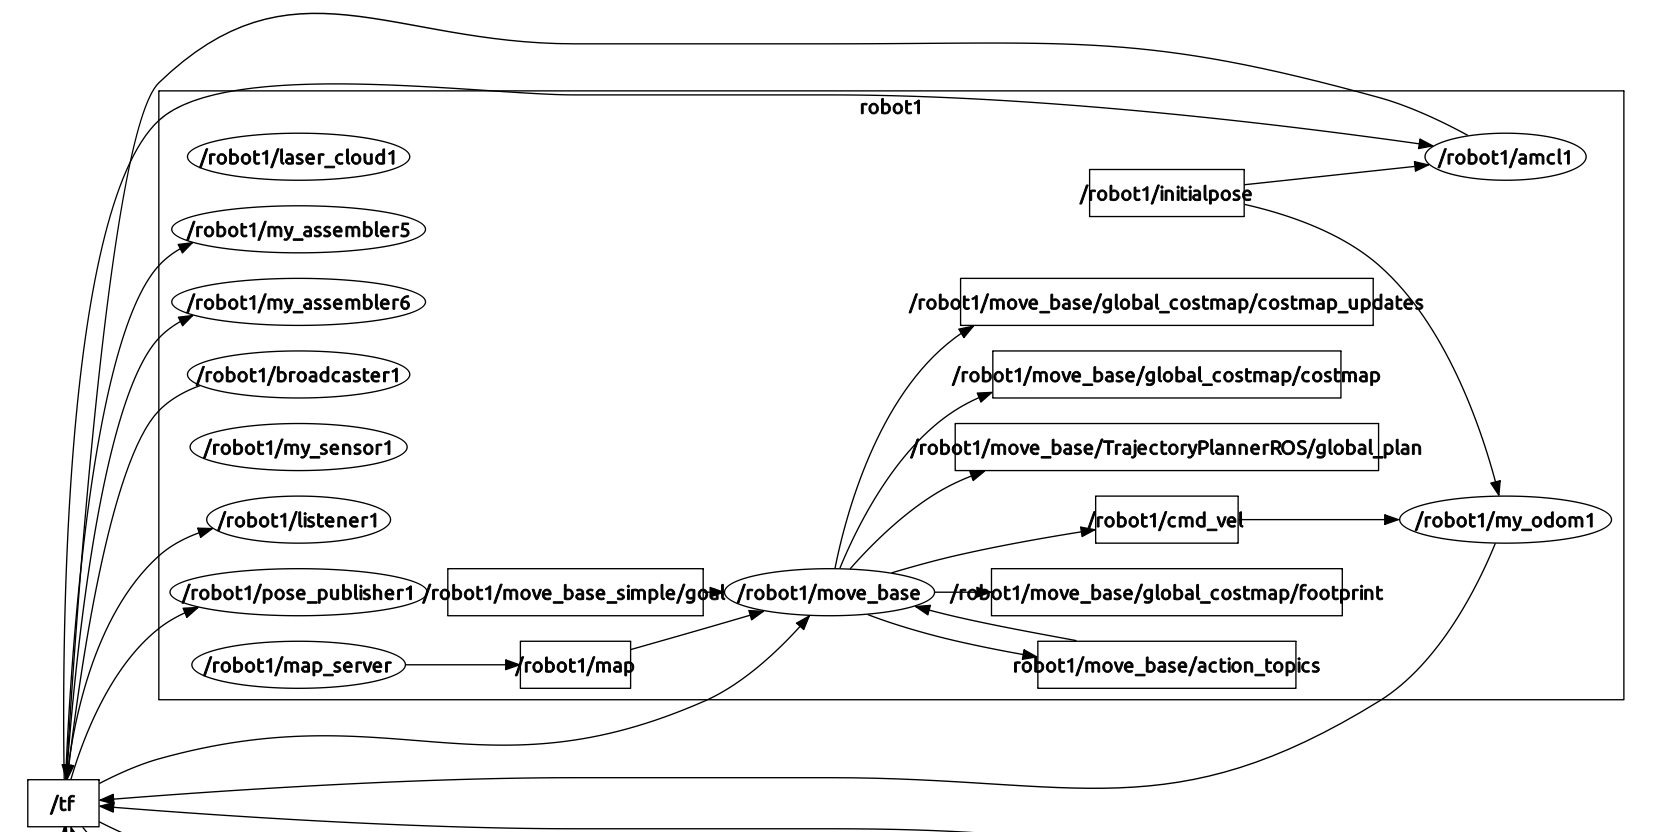
\includegraphics[width=1\hsize]{figures/ROSmapping.png}}
              \caption{Mapping of packages for a single robot.}
            \end{figure}
          \end{landscape}

        This figure is only limited to topics that at the time of producing the graph were active. Several topics start to only publish at certain point like when a goal was reached so it goes to show how useful the launch files are and how many windows would otherwise had to be created to run all the topics separately.

        As previously stated ROS uses mapping to map certain topics to each other to be able to make sense of the data. Topics are generally nodes that publish any sort of data or can even be physical objects that map from one to another. This can for instance be mapping a robot hand to the body. This means that including a mapping graph gives a great deal of the implementation in the environment. The mapping graph however does not show which topics listen or publish data from and to each other and that's why in the previous figure, there is no connection between the goal node and the outside(not visible on this figure) controller node that would actually send data through about where the robot should go. Such graphs would be extremely complex and at larger levels unreadable.

        This figure then, was also included in the project to demonstrate the architecture behind how singular robots work inside the ROS environment. It lists every class developed in the Robot package along with those pre-build by ROS to aid in simulation. Perhaps the most important package inside the environment is the Odometry package that will be discussed further in the next section.

      \subsubsection{Odometry}
        Odometry is the use of data from sensors in robots to estimate their position in the environment. The location can never be exact as some things like slide or drag or friction when the robot is moving could slow it down causing a the estimation to go off if it doesn't take those into account and even then, the location will not be as accurate. In the simulation environment, this odometry can be considered to be very accurate and in the simulation package, odometry does very little in terms of robot estimation. This package in ROS, when ran is actually mostly used to collect velocity controls from the amcl that does the localization.

        AMCL is a probabilistic localization system for robots moving in 2D that implements a monte carlo localization approach through the use of particle filters. The science behind it is very complex and the implementation is done in ROS and available as a given package. As such it is unnecessary to further mention it than to explain that it is used for main planning using the map given and publishes velocities that the robots should take to ensure that it is in the correct position and that the amcl can follow its path.

        With this information, it is easy to infer that the odometry package for this project in ROS is responsible for accepting velocities and upgrading the robots pose by this estimation. Through that, it does follow the principle of holding the position but rather than the estimation mentioned in the definition, in the environment that is used as simulation this figure is much more precise.

        Odometry is also responsible for mapping of several topics and as such, it is one of the packages that is both a subscriber and a publisher. It subscribes to messages regarding velocities and publishes mapping required for the robot to move along the map and be visible to both the visualization software as well as amcl and move\_base that are responsible for implementing robot goals functionality. Some of these move\_base packages and amcl topics can be seen on figure 5.1.

        To make the odometry applicable to all the robots separately, there was a function implemented called getName that produces topic names based on the number received from the arguments. This simplistic approach allows for the same odometry node to be reproduced saving a lot of time with coding and compiling multiple odometries for each robot separately.

        For any future developers, it is important to note that Odometry that is present in the ROS Wiki pages at the time of writing the report does not implement any of the listening and publishing. It also moves the robot forward without any command given. There is even a lack of mapping the odometry to the robot which is not mentioned in the Wiki which for beginning developers might raise a lot concerns that their code is not working. This stalled the development of the environment by considerable amounts and with such a small community everything had to be worked out through trial and error.

        The next sections discuss in more detail how amcl and move\_base packages work for further understanding.

      \subsubsection{AMCL and move\_base packages}
        The amcl and move\_base packages are the packages that allow the robots to move through the plane in the current simulation environment. Without these, the robots would stand in place with no data. They connect the robot and odometry to the map and create obstacles based on the input data from the map. This in turn allows for maps to be created .png files and speeds up the process of rolling out new maps for the robots.

        They do however pose a certain difficulty when rolling out the robots. As previously stated these packages were not created to support multiple robots and they are implemented using yaml files that are static uncompiled interpreted files. This means that variable parsing is not allowed as it was with the odometry packages and separate files have to be created for separate robots. The solution to this was already discussed in previous sections.

        The move\_base package takes in five files in the current implementation all of which define the costmaps for each specific robot. This move\_base then creates the obstacles and allows the planning to be created for the robot and publishes cmd\_vel topics that were previously stated to be subscribed to by the odometry.

        This in turn creates defines the backbone for the robot environment with single robot environment explained in great detail. The next section outlines the how these packages together are taken to create a multi-robot platform.

      \subsubsection{Tf\_prefix and Multi-robot Functionality}
        It is important to note that tf\_prefix is considered deprecated in future releases of ROS due to developers not making good or any use of it with several packages starting off with the lack of support for tf\_prefix. However, it is also important to note that without it the project could not implement the multi-platform the way it did with a clean approach that allows to add robots using a simple checklist.

        The launch files in ROS take on a role of XML defined information sources for ROS to pull in and switch on nodes based on the information on them. This way rather than switching on topics like roscore and rviz, everything can be defined to be switched on automatically saving a lot of terminal windows being open. In this project, one launch file creates a two robot environment with server connections all in one terminal using only one command.

        This kind of approach using tf\_prefix allows for a list to exist that if followed to the letter will allow a developer to add a robot to the environment in an automatic way:
          \begin{itemize}
            \item Copy an existing groups XML code
            \item Increment all the arguments parsed by one
            \item Create separate local, global and common costmaps for this robot using the old ones and increment mappings by one.
            \item Direct move\_base parameters to these files
          \end{itemize}

        This short list allows for another robot to be created with ease. In the GUI all that has to happen is to increase the number of robots allowed to be selected in the source code and compile the code. This is to emphasize that the environment was created with customizability in mind. This section also summarizes in great detail the most important aspects of the implementation of the simulation environment. Further sections will discuss the challenges met along the way with implementing the simulation environment.

      \subsection{Challenges in simulation implementation}
        The implementation of this environment in 2D Ros was by far the longest process throughout this project. Due to ROS's continuous and rather violent growth a lot of Wiki's are outdated and the community tends to be very non responsive. A lot of the work that went into this had to be trial and error based with various packages working and not working through the development phases.

        Another note to make is that ROS implements its own version of a C++ compiler that does not contain all the packages that a regular user might wish to use especially when it comes to multi-threading. This became especially difficult to use when making plugins as referencing classes to each other turned out to be a very tedious and buggy process. Some plugins also turned out to spin(Ros uses spin to loop over topics and make callbacks based on each iteration) which made it impossible to subscribe directly to topics if that specific plugin was used. This made some of the development quite difficult especially the Grid Layer. Later on with testing it turned out that the Grid Layer couldn't process the information properly anyway which leads back to the point made about ROS's expanding growth and packages not being able to keep up. At the current moment ROS is an amazing architecture however at times one of its biggest challenges is that it makes it difficult for the developer to create clean readable code due to workarounds needed to push it to its full potential.

      \subsection{Final notes for Simulation Environment}
        A full implementation of the simulation environment runs using Rviz as a platform for testing whether the robots work. The navigation stack is fully implemented and accepts commands being taken in. The logging feature is switched on and ROS generally fills up on information quite fast so its absolutely essential that if used in the future, the developer should switch logging off unless they actually wish to troubleshoot. Otherwise ROS could overflow the drive quite fast after about 20-30 runs. Without logging these resources are well preserved and don't use up this much of the computers resources as no visualization software needs to be ran.

    \section{Server}
      Here I will focus on outlining the structure for the server. I will try to make it quite brief as that server package was not my implementation but I will go into some detail about possibilities it provides and the protocol it follows.

    \section{Hider}
      Currently Hider is a very static class without any GUI. I will try to develop some Hide treasure GUI for last calls. Later on I will explain its function, how the classes are broken down and reasons for choices.

    \section{User}
      Finally with all the required functionality up I will explain a bit more about how the user environment works. This will be done through various figures of classes, telling how the communication works, explaining the use of threading and design patterns to ensure that the environment is called accordingly and reasons for choosing Swing Java over JavaFX etc. etc. etc.

  \chapter{TESTING - Modes Specification and analysis (Finish this after next meeting with what is had)}
    Modes specification and analysis will focus on altering the code in such a way that will allow provision of different results. I will provide algorithms for three different modes that allow an unbiased picture that will show how human interaction and robot collaboration will influence the results. This part will definitely allow for some research work.

    \section{System against Requirements testing}
      Here I will weigh what the system managed to achieve in comparison to the requirements set out in the specification and design chapters.
    \section{ROS Testing}
      This will be testing on the ROS environment to fish out any bugs in the code to ensure that software is of quality.(Loop missing time lookups)
    \section{Server Testing}
      Testing server connections to fish out any errors for future fixes with regards to how connections are handled. (\%\%shutdown messages could be improved on). What happens when we suddenly close the server.
    \section{GUI Testing}
      Testing the GUI, resizing etc. and testing different situations(Do the dialogs pop up correctly, Can user interrupt traveling robots etc.) What happens when the GUI closes by itself.
    \section{Use Case Testing}
      Testing the full implementation when switched on the application correctly and seeing if at any point the program crashes. Do these about 5-10 times in a row and see how many times there is a problem with software(if there is any). With these results elaborate on what could be causing issues if such present and include it in future works.
    \section{Known problems}
      \subsubsection{GridLayer}
        Talk about how the environment doesn't let robots update the costmap but are rather reliant on the static map which means that at current stage they are rather reliant on the environment being unchanging. They can also overlap in their travels.
      \subsubsection{Environment mostly simulated}
        A lot of the work to create the game is simulated like energy levels and taking pictures. Elaborate on how this might pose difficulties in the future.
      \subsubsection{ROS package stack}
        Talk about how libraries and executables are very rarely properly working together and how inclusion of external classes can lead to errors. An example of this can be integrating GridLayer using robotPosition class to set new obstacles.
      \subsubsection{System currently made to run in an uninterrupted environment}
        As of right now closing either of the applications could cause an error forcing the user not to notice any error until sufficient time has passed to realize there is a fault in the system. \textbf{Will try to fix this to ping everyone occasionally or make a note that Server could notify all other nodes of one node disabling to halt all actions and ask for a restart.}
      \subsubsection{A very strict Server}
        This actually ensures that no impostors attack the server however more frequent pings could be specified for certain applications where if the application is switched off, the user will not have to wait until the server cleans out the old GUI before a new one can be switched on.
  \chapter{Evaluation (Finish along different modes for testing)}
    \section{Project Progress Evaluation at the time of report}
      This section will largely focus on evaluating the progress made during the report. It will discuss the original goals against what was achieved and what was missing in the project. What things could have been done better? What things have been done well? Why have some things not worked out quite the way they should(Think robots overlapping each other or not constantly upgrading the map or robots not proposing what rooms to go to). Also discuss the help that was reached out for and critique the ROS community as they are difficult at times. Discuss where the project could be applied? Also make a note how compared to real life this map was really small and usually robots will have much bigger environments to transverse through. This means that if time is of essence, supporting multiple robots is absolutely critical and being scalable is another issue to look at which the project did focus on in code design.

    \section{How the project compares with other research}
      Following that, discuss how this project compares to other papers previously stated in the background and as such. In what way was this project something completely different(Think humans not in the same environment as robots). How was it similar?(Think about the collaboration papers focusing on fluency). For more ask at tomorrows meeting what can be discussed here. I could also discuss the inverse property of the project against projects like Amazon Drone Delivery.

    \section{Future possibilities for expanding the project}
      Should I write something here?

      \subsubsection{Minimizing dependencies}
        Complete care was given in the project to made the code as scalable as possible through the use of non discriminating functions(Functions that apply to all robots) through Object Oriented Programming etc. But some functions in ROS do require the user to create separate file for each robot and as such, more elaborate ways could be thought of to allow a more Object Oriented approach to be taken. With that, the scalability of the project could increase to the point that it would turn more into a non-deterministic framework that allows plug-ins to be taken in.

      \subsubsection{Automatic area clustering of robots}
        Based on research done in Sensor networks, energy limitations are a huge concern there and multitude of research was carried out on maximizing the lifetime of networks. As such, motivation can be given to displacing the robots throughout the map to maximize their lifetime and guide the user better around the game. This could be done through the use of clustering algorithms for robots to negotiate on which part of the map they will focus on. In this project this will take on a bigger challenge as in some scenarios where environments are hostile robots could be lost along their path and as such two robots could agree to search regions of the map.

      \subsubsection{Start using physical robots for the Game}
        The project stopped at using simulations to run the game. In this way it is not much different than using simple game software to simulate such an environment. Creating a framework using ROS actually allows the project to transfer from simulation to real life is actually fairly straightforward with the foundations already built up. With the robot controller, all functions are sent to specific robots odometry and since odometry will always be present the next focuses in the project could be to start implementing real life robots with maps uploaded onto them.

        In such scenarios a lot of issues would be overcome with robots creating real time data and submitting them to the map as well as avoiding obstacles that could be other robots. In such a case study users would have access to robots but not see the maze themselves. It would add excitement to the game.

      \subsubsection{Expand the GUI to JavaFX}
        Currently, the GUI is built using Java Swing which in itself is a very formal language that is usually used to build business like components with little support for drawing extra objects or on panes. There are packages such as AWT but their use is widely discouraged by the community and could stall the project more.

        Instead a proposition of using JavaFX is in place. This package is slowly used more frequently to add flexibility to otherwise difficult to handle Java GUI design. In the end the projects audience is what will determine the projects quality so ensuring a solid GUI could be the way to move forward.

      \subsubsection{Add Phone support}
        While a minor feature requiring to only boot up another GUI, gaming on the phone is becoming more and more of a standard. With that in mind giving users the freedom to not carry around a laptop to events where the game might be played, using hotspot routers for the game and allowing applications to play the game on top of computers could be in fact a very useful feature. There are numerous possibilities for implementing such a feature but there are also technologies that allow writing applications that export to all phone platforms. Discussing them however falls outside of the scope of the project.

      \subsubsection{Flexibility through Multi ROS Support}
        If the environment stayed as it is, creating VM's that run multiple ROS environments and handle them accordingly could be an approach to create a gaming environment that multiple users could enjoy online whenever they would choose to wish so. Such environment would work by using name assigning and would require adding another Server node that would handle multiple instances of the current server class that would populate itself over the machines ports with sockets. 

        This would create a scalable game environment that potentially an unlimited number of users could use. This could open opportunities for competitions in the game where based on a scoring system of choice users could compete in robotics challenges that use actual real robot operating system as opposed to simulations that wouldn't otherwise give them an experience of using a \"real\" robot in its environment.
      
      \subsubsection{Deep sea exploration}
        ROS currently lacks the support for 3D path planning. This is not to say that 3D control, that is actually available but in the future, plans might extend to ros being able to support 3D path planning and then another world of opportunity will open up in Deep sea exploration. The current project allows for communication between ROS and whatever GUI is presented so its not difficult to see how inputting the right packages for such implementations could be extremely useful. Already a lot of research has been going into node deployments in deep sea and how to use these to tackle communication however, map building of deep sea ocean and understanding more about what's beneath us is an area of research that could benefit from the framework suggested in this project where robots are given coordinates through a server allowing for a customizable GUI on the side of developers for such projects.

      \subsubsection{Search-And-Rescue Scouting}
        This is actually an extension to the paper by Govindarajan\cite{Vijay} where robots would assist a person to minimize time spent in a single room during search and rescue missions. This project could be an extension to that but much rather use robots for pre-made environments that suffered some kind of trauma to weight risks of assisting certain people and search for survivors in places that have the best chance of making it out. Building maps of risky environments could give rescuers chances of creating robust plans that would maximize the number of people saved in such harsh and difficult times.

  \chapter{Conclusion (Finish this by end of April for submission and rewriting code.)}


  \begin{thebibliography}{9}

    \bibitem{Elizabeth}
      Elizabeth I. Sklar and M. Q. Azhar, Argumentation-Based Dialogue Games for Shared Control in Human-Robot Systems,
      \emph{Journal of Human-Robot Interaction, Vol. 1, No. 1, 2012, Pages 78-95. DOI 10.5898/JHRI.1.1.Tanaka}.

    \bibitem{ChangLiu}
      Chang Liu et al. Goal Inference Improves Objective and Perceived Performance in Human-Robot Collaboration, 
      \emph{Proceedings of the 15th International Conference on Autonomous Agents and Multiagent Systems (AAMAS 2016), J. Thangarajah, K. Tuyls, C. Jonker, S. Marsella (eds.), May 9–13, 2016, Singapore.}.

    \bibitem{Vijay}
      Vijay Govindarajan et al. Human-Robot Collaborative Topological Exploration for Search and Rescue Applications,
      \emph{Distributed Autonomous Robotic Systems Volume 112 of the series Springer Tracts in Advanced Robotics pp 17-32 15 Jan 2016}.

    \bibitem{Hiraki}
      Hiraki Goto et al. Human-Robot Collaborative Assembly by On-line Human Action Recognition Based on an FSM Task Mode,
      \emph{Proc. HRI-2013 Workshop on collaborative Manipulation: New challenges for robotics and HRI, Mar. 3 2013}.

    \bibitem{Fiore}
      Michelangelo Fiore, Aurelie Clodic, Rachid Alami.On Planning and Task achievement Modalities for Human-Robot Collaboration. \emph{International Symposium on Experimental Robotics (ISER 2014), Jun 2014, Marrakech, Morocco. 15p. <hal-01149109> 13 November 2015}.

    \bibitem{ChienLiang}
      Chien-Liang Fok et al. Integration and Usage of a ROS-Based Whole Body Control Software Framework
      \emph{Robot Operating System (ROS)Volume 625 of the series Studies in Computational Intelligence pp 535-563 10 February 2016}.

    \bibitem{Liang}
      Liang S Ng et al. Open source hardware and software platform for robotics and artificial intelligence applications
      \emph{IOP Conf. Series: Materials Science and Engineering 114 (2016) 012142 doi:10.1088/1757-899X/114/1/012142}.

    \bibitem{Pedro}
      Pedro Deusdado et al. An Aerial-Ground Robotic Team for Systematic Soil and Biota Sampling in Estuarine Mudflats
      \emph{Robot 2015: Second Iberian Robotics Conference Volume 418 of the series Advances in Intelligent Systems and Computing pp 15-26}.

    \bibitem{technical}
      Elizabeth I. Sklar and Simon Parsons (2015). HRT2: System Architecture Overview, version 2.1. Technical Report, Dept of Computer Science, University of Liverpool, 2015.

    \bibitem{wiki1}
      Multiple robots simulation and navigation, \emph{http://answers.ros.org/question/41433/multiple-robots-simulation-andnavigation/}.

    \bibitem{cplus}
      Discussion on C++ being platform dependent. \emph{http://stackoverflow.com/questions/11810484/why-is-c-platformdependent}.
    \bibitem{socketio}
      Socket IO website for reference. \emph{http://socket.io/}.
    \bibitem{python}
       Book: Python Programming for the Absolute Beginner, Michael Dawson, 1 Jan 2010



  \end{thebibliography}


 \end{document}